\section{Discussion}\label{discussion}

% original
Many non-trivial problems in materials science, and in science more broadly, are explained not through a single constitutive relationship, but through a combination of contributing physics.

% Figure~\ref{fig:stress} shows an artificial dataset constructed to replicate the impact of yield stress in a two-phase, solid-solution strengthened alloy system. Using a combination of composite theory for the contribution of flow stress, {\color{red} NAME} solid solution \cite{solid solution}, and Hall-Petch \cite{Hall-Petch} strengthening, the expected yield stress is
%
% \begin{equation}
% 	\sigma_y = F_v^A \sigma_f^A + F_v^B \sigma_f^B + \sum_i C_i [x_i]^{2/3} + \sum_j k_j d_j^{-1/2} + \ldots
% \end{equation}
%
% \noindent with free parameters \\[2ex]
% \begin{conditions}
% 	F_v^i  & Volume fraction of phase $i$ \\
% 	$[x_i]$  & Concentration of solute $i$ \\
% 	d_j    & Average grain diameter of phase $j$
% \end{conditions}
% \\[2ex]
% \noindent and fixed parameters \\[2ex]
% \begin{conditions}
% 	\sigma_f^i & Flow stress of phase $i$ \\
% 	C_i        & Solid solution strengthening coefficient for solute species $i$ \\
% 	k_j        & Hall-Petch strengthening coefficient for phase $j$
% \end{tabular}
% \\[2ex]

% The goal is to iteratively improve on this constitutive model, one term at a time, and monitor the effect on the residuals between the predicted yield, $\hat{\sigma_y}$ and the actual yield $\sigma_y$.
The goal of this approach is to identify the coefficients of a hypothesized constitutive relationship, coefficients that capture the specific physics of a process, through a least-squares fit between the covector space of a neural network series expansion, $\boldsymbol{\alpha}(\boldsymbol{\theta})$, which is a function of the model parameters, and the covector space of the constitutive relationship, $\boldsymbol{\beta}(C_k)$, which is a function of the physical constants of the model.

It may be useful to introduce a schematic that not only frames the hypothesis, but also graphically registers key details of the methods section of this paper.  Such a figure is presented in Figure~\ref{fig:nn-2}


\begin{figure}[htbp]
\begin{center}
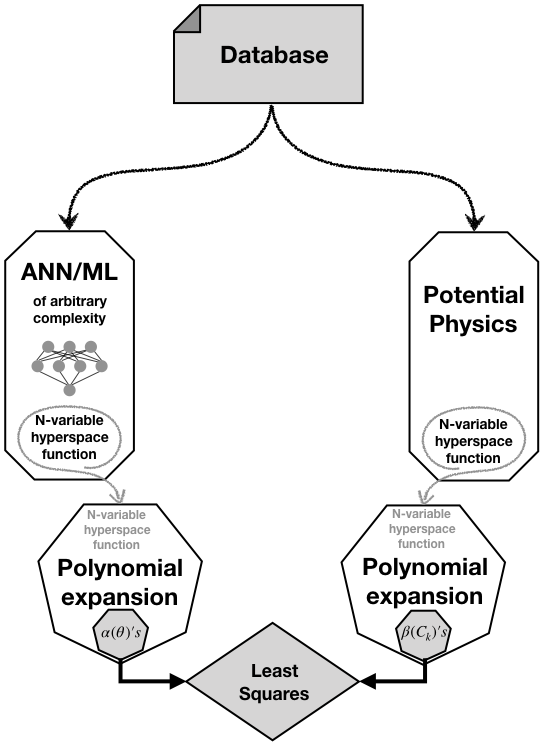
\includegraphics[width=0.4\textwidth]{fig/Schematic-02}
\caption{Schematic of the logic of the approach. The schematic could easily be expanded to show additional details and complexity on both the ANN/ML pathway and the potential physics pathway, including, for example, data selectors, physical dependencies. Similarly, the permutation of multiple architectures and postulated physics could be graphically represented, which would better represent the practical use of this approach.}
\label{fig:nn-2}
\end{center}
\end{figure}


% Find \alpha_k for neural network (NN) expansion
% Find \beta_k for constitutive relationship (CR) expansion
% Solve for C_k through fit (least-squares for now) of \alpha_k to \beta_k
Having fit the model parameters, $\boldsymbol{\theta}$, on a vector space spanned by the column vectors of ${\bf x}$, the coefficients (the covector basis) of the neural network expansion, $\boldsymbol{\alpha}(\boldsymbol{\theta})$, capture the functional relationship between the input space and the response space, both affine and non-linear contributions, introduced through those parameters, $\boldsymbol{\theta}$, and the coefficient generating functions for the activation, e.g. Equations~\ref{eqn:ReLU generating function} (Rectified Linear Unit, ReLU) and \ref{eqn:softmax generating function} (softmax), respectively.

Naturally, the activation generating functions must match the activation function chosen in the neural network model architecture. Equation~\ref{eqn:ReLU generating function} is derived for ReLU activation, the most common hidden layer activation. (Generating functions for other activations are provided in the appendix.) In addition to the hidden layers, activation functions must also be chosen for the output layer. The two most common output activations are linear (Eq.~\ref{eqn:linear generating function}) and softmax (Eq.~\ref{eqn:softmax generating function}) for regression and classification, respectively.

% ReLU activation depends on the data, others do not.
ReLU activation,
\[
    \sigma(z) = \begin{cases}
            z   & \mbox{if } z > 0, \\
            0   & \mbox{otherwise}
        \end{cases}
\]
is discontinuous in the first derivative at $z_i = 0$. Therefore, the coefficient generating function of this activation must either be either a function of the input data, ${\bf z}$ or a small modification must be made to the softplus,
\begin{equation}
    \sigma(z; \alpha) = \frac{1}{\alpha} \ln\left( 1 + e^{\alpha x} \right).
    \label{eqn:modified softmax}
\end{equation}
In the limit as $\alpha$ approaches infinity, this converges to the ReLU. Practically, though, $\alpha$ can be assigned a large value and the coefficient generating function no longer depends on the input data, see Equation~\ref{eqn:modified softplus generating function} in {\color{red} the appendix}. However, because of the high computational cost of expressing the coefficients using the modified softplus, and the relative low cost of forward evaluation of the trained neural network in order to apply Equation~\ref{eqn:ReLU generating function}, expressing the coefficient generating function of ReLU in terms of the input data, as in Equation~\ref{eqn:ReLU generating function}, rather than the training-data-agnostic approach in Equation~\ref{eqn:modified softplus generating function} would seem more practical.

% possible because \alpha and \beta both span the same subspace.
\begin{condition}
    Both the neural network and the constitutive relationship must depend on the same independent variables.
\end{condition}
That is, they must be described on the same basis vectors. The fit between the coefficients of the neural network expansion--$\boldsymbol{\alpha}$, the covector space of the neural network's basis vectors--and the coefficients of the series expansion of the constitutive relationship (its covector space, $\boldsymbol{\beta}$) is only possible because both span the same subspace and share a common description of the solution within that subspace, that is, the covector spaces are colinear. That is, suppose that $A$ maps between a vector space and its covector space. If $A: A(X) = X^*$ and $A: A(Y) = Y^*$, then $X^* = Y^*$ if and only if $X = Y$.

If ${\bf x} = ([c], d)$ are the concentration of a solute and grain size, respectively, then the constitutive relationship expansion would be,
\begin{align}
    \sigma_y &= \sigma_f  + C [c]^{2/3} + \frac{k}{\sqrt{d}} \nonumber \\
        &= \sigma_f + \underbrace{\sum_{k=0}^{\infty} a_k [c]^k}_{\text{solute}} + \underbrace{\sum_{k=0}^{\infty} b_k d^k}_{\text{Hall-Petch}} \nonumber \\
        &= \sigma_f + \sum_{k=0}^{\infty} a_k \he[\left( {\bf S}_\text{solute}{\bf x} \right)]{k} + \sum_{k=0}^{\infty} b_k \he[\left( {\bf S}_\text{Hall-Petch} {\bf x} \right)]{k}
    \label{eqn:simplified strengthening}
\end{align}
where
\begin{conditions}
    \sigma_f & Matrix flow stress. \\
    a_k & Coefficient generating function for $x^{2/3}$. \\
    b_k & Coefficient generating function for $x^{-1/2}$. \\
    {\bf S}_\text{solute} & Selection vector/matrix for choosing the solute concentration from the input vector. \\
    {\bf S}_\text{Hall-Petch} & Selection vector/matrix for choosing the grain size from the input vector.
\end{conditions}
(Coefficient generating functions can be found in Table~\ref{tab:generating functions of common functions}.) Combining Equations~\ref{eqn:simplified strengthening} and \ref{eqn:hadamard exponent vector},
\begin{multline*}
    \sigma_y = \sigma_f + \sum_{k=0}^\infty a_k \left[ \sum_{l_1=0}^k \binom{k}{l_1, l_2} \prod_{m=1}^2 (({\bf S}_\text{solute})_m {\bf x}_m)^{l_m} \right] \\
        + \sum_{k=0}^\infty b_k \left[ \sum_{l_1=0}^k \binom{k}{l_1, l_2} \prod_{m=1}^2 (({\bf S}_\text{Hall-Petch})_m {\bf x}_m)^{l_m} \right],\ l_2 = k - l_1
\end{multline*}
which further simplifies to
\begin{multline*}
    \sigma_y = \sigma_f + \sum_{k=0}^\infty \sum_{l_1=0}^k a_k \binom{k}{l_1, l_2} \prod_{m=1}^2 ({\bf S}_\text{solute})_m^{l_m} \prod_{m=1}^2{\bf x}_m^{l_m} \\
        + \sum_{k=0}^\infty \sum_{l_1=0}^k b_k \binom{k}{l_1, l_2} \prod_{m=1}^2 ({\bf S}_\text{Hall-Petch})_m^{l_m} \prod_{m=1}^2{\bf x}_m^{l_m}
\end{multline*}
such that the term $\prod_{m=1}^2{\bf x}_m^{l_m}$ serves as the common basis set over which the summation occurs, so that now, having a common basis, this simplifies to,
\begin{equation}
    \sigma_y = \sigma_f + \sum_{k=0}^\infty \sum_{l_1=0}^k \binom{k}{l_1, l_2} \left( a_k \prod_{m=1}^2 ({\bf S}_\text{solute})_m^{l_m} + b_k \prod_{m=1}^2 ({\bf S}_\text{Hall-Petch})_m^{l_m} \right) \prod_{m=1}^2{\bf x}_m^{l_m}
\end{equation}

It should be noted here that this common basis is a function of the length (dimension) of the input vector and of the order of the expansion. Therefore, two series will share the same basis vector and the same covector space if and only if they are taken to the same order. In addition, because there is no guarantee that the input vector space directions are orthogonal, there is no guarantee that the cross-term interactions will vanish and, therefore, must be included explicitly. This expansion includes all cross-terms and, through the element-wise exponentiation, also explicitly captures all combinations of powers of all cross-terms. Equation~\ref{eqn:ANN power series coefficient generating function} shows that the polynomial series expansion for the first layer of a neural network,
\[
    y^{(1)} = \sum_k \alpha^{(1)}_k \he[\left( \boldsymbol{\theta}^{(1)} {\bf x} \right)]{k},
\]
similarly relies on the element-wise exponential, $(\bullet)\he{n}$, as does the expansion of all layers. Unlike scalar exponentiation, element-wise exponentiation does not distribute, as seen in Equation~\ref{eqn:nondistributive hadamard}, and because element-wise exponentiation does not distribute, this equation explicitly captures all possible (second, $x_i^m x_j^n$; third, $x_i^m x_j^n x_k^p$; fourth, $x_i^m x_j^n x_k^p x_l^r$; etc.) cross-interactions of each term in $(\boldsymbol{\theta}{\bf x})$ at all polynomial orders. This is equivalent, then, to expanding over the basis set that includes all cross-interactions in the input vector space for both the constitutive relation and neural network polynomial expansions.

% data pre-processing
Data preprocessing is an important step in training a neural network to avoid implicit bias. Commonly, data is whitened, also known as scaling or standardization, ${\bf z}_s^{(k)}: {\bf z}_s^{(k)} = \frac{{\bf z}^{(k)} - \overline{{\bf z}^{(k)}}}{\sigma}$, where $\overline{{\bf z}^{(k)}}$ is the arithmetic mean and $\sigma$ the standard deviation of data in layer, $k$. However, a model trained on such scaled data would no longer share the vector space of the constitutive relationship. To ensure that both the neural network and constitutive relation expansions share a common vector space, and thus a common covector space, this whitening procedure must be integrated into the construction of the neural network architecture.

Procedurally, the neural network expansion proceeds as described in Section~\ref{methods}. The input to each layer, which is the output from the previous layer, is subjected first to an affine transformation, then to an activation function. The activation function is completely described though its polynomial expansion and the corresponding coefficient generating function. Using this same structure, then, data whitening can be applied to any layer, including the input layer, as an identity tranform ($\boldsymbol{\theta} = {\bf I}_d$, where $d$ is the dimension of the source layer) followed by the whitening expansion whose coefficient generating function is simply,
\begin{equation}
    \alpha_k({\bf z}) = \begin{cases}
        -\overline{\bf z}/\sigma    & \mbox{if } k = 0, \\
        1/\sigma                    & \mbox{if } k = 1, \\
        0                           & \mbox{otherwise}
    \end{cases}
\end{equation}
where
\begin{conditions}
    \overline{\bf z}    & The mean of the data into the standarization layer. \\
    \sigma              & The standard deviation of the data into the standardization layer.
\end{conditions}
By introducing such a whitening layer, data standardization can be included at any point in the neural network architecture.

% dimensional sufficiency
{\color{red} TBW. This must answer the question: how do we know if we've measured the right things--not the number of measurements, but that we have enough information? How do we know that the solution has converged? Example: A model is to be fit to the number of cakes produced by a bakery. If we are given weights of flour and sugar and number of eggs, our model can accurately tell us the \emph{volume} of cakes produced, but not the number. If this bakery makes cupcakes, but the model is trained across a spectrum of bakers, such as purveyors of wedding cakes and catering companies who work with large sheet cakes, then our dimensions (flour, sugar, eggs) are insufficient to fit the number of cakes produced. If, however, we also include number of orders and revenue, some information about the \emph{quanta} of cakes is baked into those two additional dimensions (sorry, I couldn't help myself). Therefore, a model based only on (flour, sugar, eggs) is dimensionally insufficient, but a model based on (flour, sugar, eggs, order size, revenue) is dimensionally sufficient.

This is a broader question that may be beyond the scope of this paper. Let's return to this if, after completing the first pass, we feel that this can be addressed by what we've done.}

% comment on the distance metric
% The Euclidean ($L_2\textrm{-norm}$) distance is used in optimizations, such as the training of neural networks and other machine learning algorithms, through the mean-square error,
% \begin{equation*}
%     \argmin_{\boldsymbol{\theta}} \|{\bf y} - \boldsymbol{\theta}{\bf x}\|.
% \end{equation*}
% However because of the curse of dimensionality,~\cite{curse of dimensionality reference?} the $L_2\textrm{-norm}$ is not a desirable metric in high-dimensional spaces.

This leads to a seven-step process for systematically and incrementally extracting physics information from an ANN:
\begin{enumerate}
	\item Collect data--features and targets--for which relationships are expected to exist.
	\item Design and train a fully dense multi-layer perceptron network (ANN).
	\item Build a power series expansion from the architecture of this ANN, using Equations~(\ref{eqn:sigmoid zeta expansion}) and (\ref{eqn:ANN power series coefficient generating function}) to populate the coefficients using the trained weights from the neural network.
	\item Hypothesize a constitutive relationship between the feature space and the target space. \label{item:hypothesis}
	\item Recast the terms in the hypothesis function from \#\ref{item:hypothesis} as power series expansions, creating power series coefficient generating functions that are functions of the constitutive model fitting parameters. An example of this process is provided below, and a table of select power series expansions relevant to materials research are provided in Table~(\ref{table:power series expansions}). \label{item:coefficients}
	\item Perform an optimization, \emph{e.g.} least squares, fit to find the fitting parameters from \#\ref{item:coefficients}
	\item Calculate the residuals of the ANN power series expansion coefficient vector, and from this residual vector, the error in the model. If the accuracy is sufficient for the application, stop; otherwise, expand the constitutive relationship from step \#\ref{item:hypothesis} and repeat.
\end{enumerate}


%\noindent {\color{red} How does dropout affect this? It doesn't. Dropout simply sets specific $\boldsymbol\theta$ to zero, which is handled seamlessly in the previous treatment.}


% ----- POWER SERIES COEFFICIENT DERIVATION ----- %
We can represent the recursive structure of a neural network as a series of transformations on a particular power series. Using this method, we are able to write an algorithm that will compute the coefficients of a power series determined by some neural network up to some order of approximation. We tackle this in two steps to illuminate the properties of this solution. First, we describe the problem in a scalar sense where the interpretation is easy to understand and the solution is comprehensible. Second, we derive a vector approach that would be used in the case of a typical neural network which has more intricate and less obvious details. We describe each of these scenarios purely mathematically so that this derivation may be used for machine learning methods other than neural networks.

\section{Scalar Transformation}

\subsection{Notation}
Suppose that $x \in \mathbb{R}$ is a scalar, $y \in \mathbb{R}$ is a scalar, $\theta \in \mathbb{R}$ is a scalar, and $\sigma: \mathbb{R} \to \mathbb{R}$ is an analytic function. Since $\sigma$ is analytic, it can be represented as

\begin{align*}
    \sigma(x)
    &= s_0 + s_1 x + s_2 x^2 + \cdots \\
    &= \sum_{k=0}^{\infty} s_{k} x^{k}.
\end{align*}

Suppose that we can represent $x$ as a power series of another scalar $z$.

\begin{align*}
    x
    &= a_0 + a_1 z + a_2 z^2 + \cdots \\
    &= \sum_{n=0}^{\infty} a_{n} z^{n}.
\end{align*}

Finally, suppose that we have the relation

\begin{equation*}
    y = \sigma(\theta x)
\end{equation*}

\subsection{Objective}
We want to represent $y$ as a power series of $z$.

\begin{align*}
    y
    &= b_0 + b_1 z + b_2 z^2 + \cdots \\
    &= \sum_{n=0}^{\infty} b_{n} z^{n}
\end{align*}

We will rewrite the expression for $y$ to find these coefficients $b_i$ for $i = 0, 1, 2, \ldots$

\begin{align*}
    y
    &= \sigma(\theta x) \\
    &= \sum_{k=0}^{\infty} s_k (\theta x)^k \\
    &= \sum_{k=0}^{\infty} s_k \left(\theta \sum_{n=0}^{\infty} a_{n} z^{n}\right)^{k} \\
    &= \sum_{k=0}^{\infty} s_k \theta^k \left(\sum_{n=0}^{\infty} a_{n} z^{n}\right)^{k} \\
    &= \sum_{k=0}^{\infty} s_k \theta^k \left(\sum_{k_0 + k_1 + k_2 + \cdots = k} \binom{k}{k_0, k_1, k_2, \cdots} \prod_{n=0}^{\infty} (a_n z^{n})^{k_n} \right)
\end{align*}

\subsection{Coefficient Extraction}

To extract the coefficient $b_i$ from the previous equation, we must find terms satisfying 

\begin{align*}
    i
    &= 0 k_0 + 1 k_1 + 2 k_2 + \cdots \\
    &= \sum_{n=0}^{\infty} n k_n
\end{align*}

and

\begin{align*}
    k
    &= k_0 + k_1 + k_2 + \cdots \\
    &= \sum_{n=0}^{\infty} k_n
\end{align*}

If satisfying both of these conditions, then the value

\begin{equation*}
    s_k \theta^k \binom{k}{k_0, k_1, k_2, \cdots} \prod_{n=0}^{\infty} a_n^{k_n}
\end{equation*}

is added to the sum of $b_i$. In concise terms we formulate

\begin{align*}
    b_i
    &= \sum_{k=0}^{\infty} s_k \theta^k \sum_{\substack{k_0 + k_1 + k_2 + \cdots = k \\ 0 k_0 + 1 k_1 + 2 k_2 + \cdots = i}} \binom{k}{k_0, k_1, k_2, \cdots} \prod_{n=0}^{\infty} a_n^{k_n} \\
    &= \sum_{k=0}^{\infty} s_k \theta^k \sum_{\substack{k_0 + k_1 + k_2 + \cdots + k_i = k \\ 0 k_0 + 1 k_1 + 2 k_2 + \cdots + i k_i = i}} \binom{k}{k_0, k_1, k_2, \cdots, k_i} \prod_{n=0}^{\infty} a_n^{k_n} 
\end{align*}

\subsection{Worked Coefficients}

We can find $b_0$. $i = 0 \implies k_1 = k_2 = \cdots = 0$ so $k_0 = k$. Therefore,

\begin{align*}
    b_0 
    &= \sum_{k=0}^{\infty} s_k \theta^k \sum_{\substack{k_0 + k_1 + k_2 + \cdots = k \\ 0 k_0 + 1 k_1 + 2 k_2 + \cdots = 0}} \binom{k}{k_0, k_1, k_2, \cdots} \prod_{n=0}^{\infty} a_n^{k_n} \\
    &= \sum_{k=0}^{\infty} s_k \theta^k \binom{k}{k} a_0^{k} \\
    &= \sum_{k=0}^{\infty} s_k \theta^k a_0^k
\end{align*}

We can also find $b_1$. $i = 1 \implies k_1 = 1, k_2 = k_3 = \cdots = 0$ so $k_0 = k - 1$ and $k_1 = 1$. Therefore,

\begin{align*}
    b_1
    &= \sum_{k=0}^{\infty} s_k \theta^k \sum_{\substack{k_0 + k_1 + k_2 + \cdots = k \\ 0 k_0 + 1 k_1 + 2 k_2 + \cdots = 1}} \binom{k}{k_0, k_1, k_2, \cdots} \prod_{n=0}^{\infty} a_n^{k_n} \\
    &= \sum_{k=0}^{\infty} s_k \theta^k \binom{k}{k - 1, 1} a_0^{k - 1} a_1 \\
    &= \sum_{k=0}^{\infty} k s_k \theta^k a_0^{k-1} a_1
\end{align*}

We can also find $b_2$, but the formulation is slightly more complicated. 

\begin{itemize}
    \item $i = 2 \implies k_3 = k_4 = k_5 = \cdots = 0$ and
    \begin{itemize}
        \item $k_2 = 0, k_1 = 2, k_0 = k - 2$ or
        \item $k_2 = 1, k_1 = 0, k_0 = k - 1$
    \end{itemize}
\end{itemize}

Therefore,

\begin{align*}
    b_2
    &= \sum_{k=0}^{\infty} s_k \theta^k \sum_{\substack{k_0 + k_1 + k_2 + \cdots = k \\ 0 k_0 + 1 k_1 + 2 k_2 + \cdots = 2}} \binom{k}{k_0, k_1, k_2, \cdots} \prod_{n=0}^{\infty} a_n^{k_n} \\
    &= \sum_{k=0}^{\infty} s_k \theta^k \left(\binom{k}{k - 2, 2, 0}a_0^{k-2} a_1^{2} + \binom{k}{k - 1, 0, 1}a_0^{k-1} a_2\right) \\
    &= \sum_{k=0}^{\infty} s_k \theta^k \left(\frac{k(k-1)}{2} a_0^{k-2}a_1^{2} + k a_0^{k-1}a_2\right)
\end{align*}

Note that when calculating $b_i$, the value of $i$ constrains $k_{i+1} = k_{i+2} = \cdots = 0$. Also, $k_1, k_2 \cdots, k_i$ are finite and $k_0 = k - k_1 - k_2 - \cdots - k_i$.

\section{Vector Transformation}
\subsection{Notation}

Suppose that $\mathbf{x} \in \mathbb{R}^d, (d \in \mathbb{Z})$ is a vector, $\mathbf{y} \in \mathbb{R}^c, (c \in \mathbb{Z})$ is a vector, $\mathbf{\Theta} \in \mathbb{R}^{c \times d}$ is a matrix, and $\sigma: \mathbb{R} \to \mathbb{R}$ is an analytic function. Since $\sigma$ is analytic, it can be represented as

\begin{align*}
    \sigma(x)
    &= s_0 + s_1 x + s_2 x^2 + \cdots \\
    &= \sum_{k=0}^{\infty} s_{k} x^{k}.
\end{align*}

Suppose that we can represent each entry of $\mathbf{x}$ as a power series of the entries of a vector $\mathbf{z} \in \mathbb{R}^{w}, (w \in \mathbb{Z})$.

\begin{align*}
    \forall i &= 1, \cdots, d, \\ x_i
    &= a^{(i)}_{0,0,\cdots,0} + a^{(i)}_{1,0,\cdots,0} z_1 + a^{(i)}_{2,0,\cdots,0} z_1^2 + \cdots \\
    &+ a^{(i)}_{0,1,\cdots,0} z_2 + a^{(i)}_{1,1,\cdots,0} z_1 z_2 + a^{(i)}_{2,1,\cdots,0} z_1^2 z_2 + \cdots \\
    &+ a^{(i)}_{0,0,\cdots,1} z_w + a^{(i)}_{1,0,\cdots,1} z_1 z_w + a^{(i)}_{2,0,\cdots,1} z_1^2 z_w + \cdots \\
    &= \sum_{n_1,n_2,\cdots,n_w}^{\infty,\infty,\cdots,\infty} a^{(i)}_{n_1,n_2,\cdots,n_w} z_1^{n_1} z_2^{n_2} \cdots z_w^{n_w}.
\end{align*}

Finally, suppose that we have the relation

\begin{equation*}
    \mathbf{y} = \circ\sigma(\mathbf{\Theta} \mathbf{x})
\end{equation*}

where $\circ\sigma: \mathbb{R}^{c} \to \mathbb{R}^{c}$ is the $\sigma$ function applied element-wise to a vector.

\subsection{Objective}
We want to represent each entry of $\mathbf{y}$ as a power series of the entries of $\mathbf{z}$.

\begin{align*}
    \forall i &= 1, \cdots, c, \\ y_i
    &= b^{(i)}_{0,0,\cdots,0} + b^{(i)}_{1,0,\cdots,0} z_1 + b^{(i)}_{2,0,\cdots,0} z_1^2 + \cdots \\
    &+ b^{(i)}_{0,1,\cdots,0} z_2 + b^{(i)}_{1,1,\cdots,0} z_1 z_2 + b^{(i)}_{2,1,\cdots,0} z_1^2 z_2 + \cdots \\
    &+ b^{(i)}_{0,0,\cdots,1} z_w + b^{(i)}_{1,0,\cdots,1} z_1 z_w + b^{(i)}_{2,0,\cdots,1} z_1^2 z_w + \cdots \\
    &= \sum_{n_1,n_2,\cdots,n_w}^{\infty,\infty,\cdots,\infty} b^{(i)}_{n_1,n_2,\cdots,n_w} z_1^{n_1} z_2^{n_2} \cdots z_w^{n_w}.
\end{align*}

We will rewrite the expression for $y_i$ to find these coefficients $b^{(i)}_{n_1, n_2, \cdots, n_w}$ for $(n_1, n_2, \cdots, n_w)$ from $(0, 0, \cdots, 0)$ to $(\infty, \infty, \cdots, \infty)$.

\begin{align*}
    \forall i &= 1, \cdots, c, \\ y_i
    &= \left[\circ\sigma(\mathbf{\Theta} \mathbf{x})\right]_i \\
    &= \sigma(\left[\mathbf{\Theta} \mathbf{x}\right]_i) \\
    &= \sigma(\mathbf{\theta}_i \mathbf{x}) \\
    &= \sum_{k=0}^{\infty} s_k (\mathbf{\theta}_i \mathbf{x})^k \\
    &= \sum_{k=0}^{\infty} s_k \left(\sum_{j=1}^{d} \theta_{ij} x_{j}\right)^k \\
    &= \sum_{k=0}^{\infty} s_k \left(\sum_{k_1 + \cdots + k_d = k} \binom{k}{k_1, \cdots, k_d} \prod_{j=1}^{d} (\theta_{ij} x_j)^{k_j} \right) \\
    &= \sum_{k=0}^{\infty} s_k \left(\sum_{k_1 + \cdots + k_d = k} \binom{k}{k_1, \cdots, k_d} \prod_{j=1}^{d}\theta_{ij}^{k_j} \left(\sum_{n_1, \cdots, n_w}^{\infty,
    \cdots, \infty} a^{(j)}_{n_1,\cdots,n_w} z_1^{n_1}  \cdots z_w^{n_w} \right)^{k_j}\right) \\
    &= \sum_{k=0}^{\infty} s_k \left(\sum_{k_1 + \cdots + k_d = k} \binom{k}{k_1, \cdots, k_d} \prod_{j=1}^{d} \theta_{ij}^{k_j} \left(\sum_{\sum [l] = k_j} \binom{k_j}{[l]} \prod_{n_1, \cdots, n_w}^{\infty, \cdots, \infty} (a^{(j)}_{n_1, \cdots, n_w} z_1^{n_1} \cdots z_w^{n_w})^{l_{n_1, \cdots, n_w}} \right)\right)
\end{align*}

where

\begin{align*}
    [l] = l_{\underbrace{0, \cdots, 0}_{\times w}}, \ldots, l_{\underbrace{\infty, \cdots, \infty}_{\times w}}
\end{align*}

\subsection{Coefficient Extraction}

To extract the coefficient $b^{(i)}_{m_1, \cdots, m_w}$ from the previous equation, we must find terms satisfying index constraints

\begin{align*}
    k_1 + k_2 + \cdots + k_d &= k \\
    l_{0, \cdots, 0} + \cdots + l_{\infty, \cdots, \infty} &= k_j
\end{align*}

and power constraints

\begin{align*}
    \sum_{n_1, \cdots, n_w}^{\infty, \cdots, \infty} n_1 l_{n_1, \cdots, n_w} &= m_1 \\
    \sum_{n_1, \cdots, n_w}^{\infty, \cdots, \infty} n_2 l_{n_1, \cdots, n_w} &= m_2 \\
    \vdots \qquad &= \;\; \vdots \\
    \sum_{n_1, \cdots, n_w}^{\infty, \cdots, \infty} n_w l_{n_1, \cdots, n_w} &= m_w.
\end{align*}

Notice that the power constraints can be simplified slightly since any solution must also satisfy

\begin{equation*}
    l_{n_1, \cdots, n_{p-1}, m_p + 1, n_{p+1}, \cdots, n_w} = l_{n_1, \cdots, n_{p-1}, m_p + 2, n_{p+1}, \cdots, n_w} = \cdots = 0
\end{equation*}

resulting in

\begin{align*}
    \sum_{n_1, \cdots, n_w}^{m_1, \cdots, m_w} n_1 l_{n_1, \cdots, n_w} &= m_1 \\
    \sum_{n_1, \cdots, n_w}^{m_1, \cdots, m_w} n_2 l_{n_1, \cdots, n_w} &= m_2 \\
    \vdots \qquad &= \;\; \vdots \\
    \sum_{n_1, \cdots, n_w}^{m_1, \cdots, m_w} n_w l_{n_1, \cdots, n_w} &= m_w.
\end{align*}

If satisfying all of these constraints, then the value

\begin{equation*}
    s_k \binom{k}{k_1, \cdots, k_d} \binom{k_j}{[l]} \theta_{ij}^{k_j} (a^{(j)}_{n_1, \cdots, n_w})^{l_{n_1, \cdots, n_w}}
\end{equation*}

is added to the sum of $b^{(i)}_{m_1, \cdots, m_w}$. In concise terms we formulate

\begin{align*}
    b^{(i)}_{m_1, \cdots, m_w} = \sum_{k=0}^{\infty} s_k \sum_{k_1 + \cdots + k_d = k} \binom{k}{k_1, \cdots, k_d} \prod_{j=1}^{d} \theta_{ij}^{k_j} \sum_{\substack{l_{0, \cdots, 0} + \cdots + l_{\infty, \cdots, \infty} = k_j \\ \sum_{n_1, \cdots, n_w}^{m_1, \cdots, m_w} n_1 l_{n_1, \cdots, n_w} = m_1 \\ \vdots \\ \sum_{n_1, \cdots, n_w}^{m_1, \cdots, m_w} n_w l_{n_1, \cdots, n_w} = m_w}} \binom{k_j}{[l]} (a^{(j)}_{n_1, \cdots, n_w})^{l_{n_1, \cdots, n_w}}
\end{align*}

The only issue is that of finding solutions to the constraints.

\subsection{Interpretation}

We can use this method for deriving power series for repeatedly composed functions with linear transformations (i.e. $\mathbf{y} = f(\mathbf{\Theta}_3 f(\mathbf{
\Theta}_1 f(\mathbf{\Theta}_1 \mathbf{x})))$). We represent our original input variable as $\mathbf{x} = \mathbf{z}$ so that we have coefficients $a_{1, 0, \cdots, 0} = a_{0, 1, \cdots, 0} = \cdots = a_{0, 0, \cdots, 1} = 1$ with all other coefficients zero. Then, we update $\mathbf{a}$ each composition of the function to obtain $\mathbf{b}$ for $\mathbf{y}$. This can be easily applied to neural networks.

\vspace{0.10in}
\noindent
In order to make this method computationally feasible, we must truncate the power series at some precision. Say the maximum power we wish on any variable is $K$, then, we simply replace instances of $\sum_{k=0}^{\infty} s_k x^k$ with $\sum_{k=0}^{K} s_k x^k$. This works because our power constraints limit the maximum powers of our variable. Thus, coefficients of order $0, 1, \cdots, K$ will have no error and our approximation will only have truncation error from dropping terms with order $> K$.

\subsection{Constraint Analysis}

The constraints are of a form of a restricted partition within number theory. There is literature concerning these exact constraints (see https://arxiv.org/pdf/1611.09931.pdf). We can construct an algorithm that operates in $\mathcal{O}(K^w)$ time by looping each indices $l_{0, \cdots, 0}, \cdots, l_{m_1, \cdots, m_w}$ from $0$ to $K$ and checking if they satisfy the constraints. This warrants some future study to see if there are ways to reduce the operation time and find solutions to the system of constraints more quickly.